%!TEX root = project.tex

\chapter*{About this project}
\paragraph{Abstract}
The aim of this project is to create a multiplatform game that can be played through a virtual reality headset, gaming desktop and also using a mobile device. In the following documentation we will examine and explorer how we conducted this project and also the improvements we would suggest, if the project were to continue. For the virtual reality headset we used the Oculus Rift CV1 head mounted display, controls and sensors. For the mobile devices we used a Samsung smartphone running an android operating system and a Lenovo Yoga Book tablet for implementation. The idea for the game came from Bandai Namco's release of Mario Kart VR. This game is released only as an arcade model, it is not available for the mass market or any home user model, so we decide to create a similar style game. We styled our game on the hit TV show Ricky and Morty, this was simply an aesthetic choice to keep the game within the same genre and similar style of Mario Kart.

\paragraph{Authors}
The authors of this Document are Michael Kidd, Kevin Moran, John Mannion and Ray Mannion.

\chapter{Introduction}
The introduction should be about three to five pages long.

https://www.roadtovr.com/mario-kart-vr-comes-us-today-bandai-namcos-newest-vr-arcade/~\cite{Bandai Namco}

Make sure you use references~\cite{einstein}

\chapter{Context}
\begin{itemize}
\item Provide a context for your project.
\item Set out the objectives of the project
\item Briefly list each chapter / section and provide a 1-2 line description of what each section contains.
\item List the resource URL (GitHub address) for the project and provide a brief list of the main elements at the URL.
\end{itemize}

\section{Filler}

\subsection{More filler}

\section{Filler}

\chapter{Methodology}
About one to two pages.
Describe the way you went about your project:

\begin{itemize}
\item Agile / incremental and iterative approach to development. Planning, meetings.
\item What about validation and testing? Junit or some other framework.
\item If team based, did you use GitHub during the development process.   Yes we did!!!!!!
\item Selection criteria for algorithms, languages, platforms and technologies.
\end{itemize}
Check out the nice graphs in Figure \ref{tikz:graphs}, and the nice diagram in Figure \ref{tikz:mydiagram}.

\begin{figure}
  \centering
  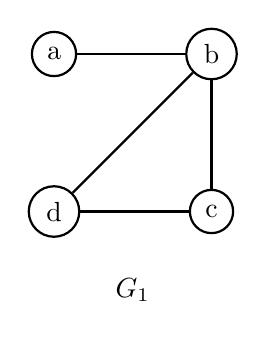
\begin{tikzpicture}
  \begin{scope}[every node/.style={circle,thick,draw}]
  \node (a) at (0,2) {a};
  \node (b) at (2,2) {b};
  \node (c) at (2,0) {c};
  \node (d) at (0,0) {d};
  \end{scope}
  \begin{scope}[every edge/.style={draw=black,thick}]
  \path (a) edge (b);
  \path (b) edge (c);
  \path (b) edge (d);
  \path (c) edge (d);
  \end{scope}
  \node () at (1,-1) {$G_1$};
  \end{tikzpicture}
  \hspace{1.5cm}
  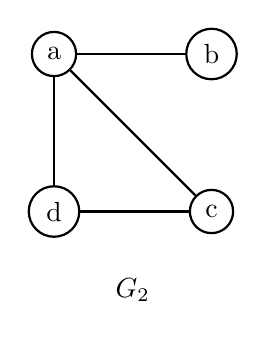
\begin{tikzpicture}
  \begin{scope}[every node/.style={circle,thick,draw}]
  \node (1) at (0,2) {a};
  \node (2) at (2,2) {b};
  \node (3) at (2,0) {c};
  \node (4) at (0,0) {d};
  \end{scope}
  \begin{scope}[every edge/.style={draw=black,thick}]
  \path (1) edge (2);
  \path (1) edge (3);
  \path (1) edge (4);
  \path (3) edge (4);
  \end{scope}
  \node () at (1,-1) {$G_2$};
  \end{tikzpicture}
  \caption{Nice pictures}
  \label{tikz:graphs}
\end{figure}


\begin{figure}
  \centering
  \begin{tikzpicture}[node distance=6cm]
  \node (a) [rect] {A Big Blue Block};
  \node (b) [oval, right of=a] {And His Oval Friend};
  \draw [line] (a) -- (b);
  \end{tikzpicture}
  \caption{Nice pictures}
  \label{tikz:graphs}
\end{figure}


\chapter{Technology Review}
About seven to ten pages.
\begin{itemize}
\item Describe each of the technologies you used at a conceptual level. Standards, Database Model (e.g. MongoDB, CouchDB), XMl, WSDL, JSON, JAXP.
\item Use references (IEEE format, e.g. [1]), Books, Papers, URLs (timestamp) – sources should be authoritative. 
\end{itemize}

\section{XML}
Here's some nicely formatted XML:
\begin{minted}{xml}
<this>
  <looks lookswhat="good">
    Good
  </looks>
</this>
\end{minted}

\chapter{System Design}
As many pages as needed.
\begin{itemize}
\item Architecture, UML etc. An overview of the different components of the system. Diagrams etc… Screen shots etc.
\end{itemize}

\begin{table}[h]
  \centering
  \begin{tabular}{x{2cm}p{3cm}}
    \toprule \\
    Column 1 & Column 2 \\
    \midrule \\
    Rows 2.1 & Row 2.2 \\
    \bottomrule
  \end{tabular}
  \caption{A table.}
  \label{table:mytable}
\end{table}

\chapter{System Evaluation}
As many pages as needed.
\begin{itemize}
\item Prove that your software is robust. How? Testing etc. 
\item Use performance benchmarks (space and time) if algorithmic.
\item Measure the outcomes / outputs of your system / software against the objectives from the Introduction.
\item Highlight any limitations or opportuni-ties in your approach or technologies used.
\end{itemize}

\chapter{Conclusion}
About three pages.

\begin{itemize}
\item Briefly summarise your context and ob-jectives (a few lines).
\item Highlight your findings from the evalua-tion section / chapter and any opportuni-ties identified.
\end{itemize}

